\chapter{Agent for StarCraft II}

In this chapter we first provide a birds-eye view of the implemented model architecture. We then dive deeper into two key aspects: categorical feature embeddings and action policies with multiple outputs. These aspects are not only critical to the whole agent, but also neither present in other common benchmark environments such as Atari and MuJoCo, nor described in-depth in the reference publication. Finally, we describe some of the important implementation details such as platform choice and codebase structure.

\section{Model Architecture}

Agent model architecture closely follows FullyConv architecture description from the SC2LE paper and visualized in Figure~\ref{fig:arch} below. The name FullyConv refers to the fully convolutional, resolution preserving nature of the model, remaining spatial in structure from beginning to the end. This approach is in contrast with typical usages of convolutional layers, that reduce in size at each layer, ending with a conversion to a flat vector with dense layer on top (ex. Atari DQN architecture~\cite{Mnih2015}).
\\\\
The need for spatial structure preserving architecture stems from the nature of the environment and how an agent typically interacts with it. A significant part of navigating StarCraft comes in the form of mouse clicks, either directly on the game screen or on the minimap. For this reason it would be beneficial for the spatial policies to remain in the same domain space as the incoming spatial features~\cite{Vinyals2017}.
\\\\
The model begins with three essentially separate blocks, representing different sources of information: two for spatial data (screen and minimap) and one for non-spatial data. First two sources represent the spatial data that an agent could see on the screen or on the minimap respectively (ex. unit type or health), whereas non-spatial data stands for additional information a player can get about the game state, such as number of resources or army count. 
\\\\
Spatial information inputs consist of $n \times n$ pixel “images”, where each pixel represents value of the feature at a given pixel. Since most units are larger than a pixel in size, the information about them is duplicated across every pixel they occupy.
\\\\
Spatial inputs are passed through two convolutional layers with $5\times5$, $3\times3$ size and $16$, $32$ filter count respectively. In order to preserve resolution, these layers have stride 1 and are evenly padded. Non-spatial inputs are logarithmically scaled and then broadcasted to the same dimensions as spatial inputs -- that is, the information is repeated across every pixel in the image to match height and width of the spatial features.
\\\\
The three blocks are then merged into a single $H\times W \times D$ state representation. From here the state is converted into a spatial policy, non-spatial policy and value estimate of the current state. Spatial policy conversion is done by applying one 1$\times$1 convolutional layer with a single output filter. For non-spatial policy and value estimates the state is first pushed through a joint fully connected (FC) layer and then another final FC layer representing the policy and value estimate.
\\\\
A final softmax layer is applied to action policy outputs to obtain probability distributions. Action policies are described in greater detail in section 2.1.2.

\begin{figure}[ht]
\begin{center}
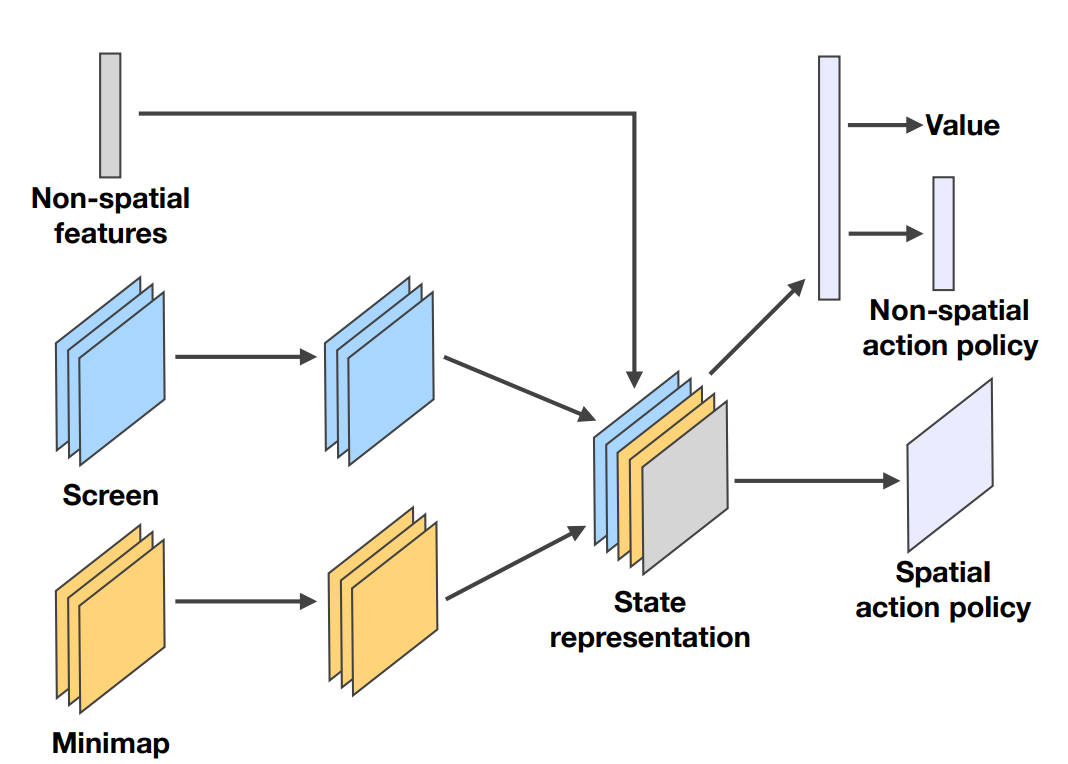
\includegraphics[width=0.9\textwidth]{arch}
\caption{FullyConv architecture as described and illustrated in~\cite{Vinyals2017}.}
\label{fig:arch}
\end{center}
\end{figure}

\subsection{Embedding Layer}

One special type of input information are the categorical spatial features, which represent some categorical data for every pixel in the feature ``image''. For example, a unit could be represented by $n \times m$ pixel grid and every pixel in this grid would contain various information about this unit, such as its type (ex. marine, worker) or id of the player than controls him. As these features are not ordinal in nature, they can not be simply processed as is. One typical way to handle such situation is to apply one-hot expansion to a dimension that matches the number of categorical levels of the feature. 
\\\\
In case of spatial features naive one-hot expanding would be prohibitively expensive from computational perspective. For example the unit type feature has over 1800 levels, which would result in a $H \times W \times 1800$ sized tensor just on the input layer. For this reason, the one-hot expanded tensor must be reduced in the channel dimension back to a reasonable level (to continuous space in the SC2LE paper) with 1$\times$1 convolutional layer (see Figure~\ref{fig:embed}). Intuitively, this layer has a separate parameter responsible for recognizing different categorical levels of a given feature. Since input to the layer is a one-hot expanded tensor, an output will consist of an “image” where each pixel is filled with the relevant parameters value.

\begin{figure}[ht]
\begin{center}
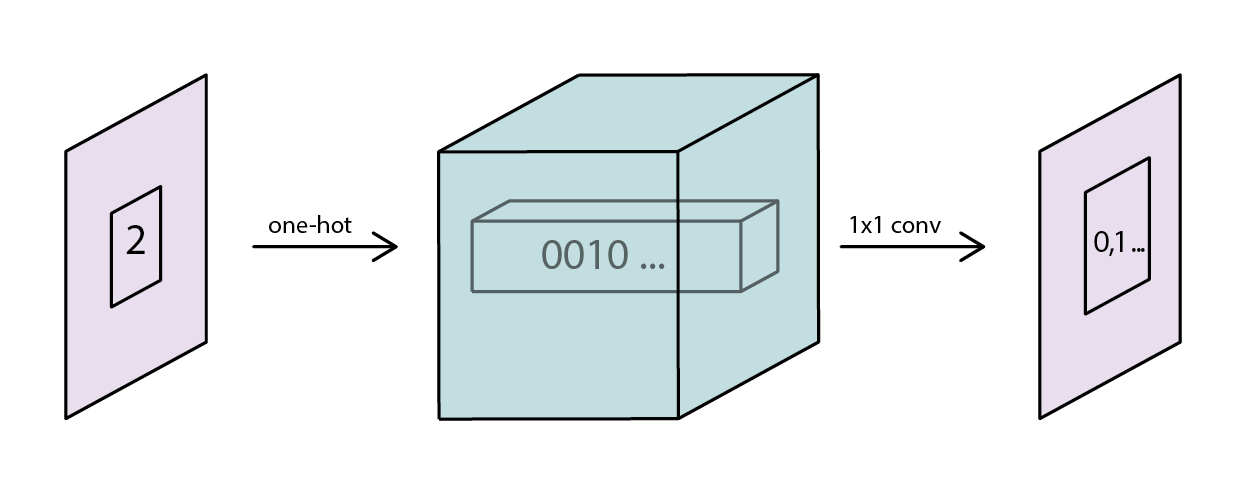
\includegraphics[width=\textwidth]{embed}
\caption{Embedding layer visualization. An input image of $H \times W \times 1$ size with value 2 at a specified pixel is first one-hot expanded, producing an $H \times W \times C$ tensor with all zeros except for 1 at index 2 for specified pixel’s vector. Resulting tensor is then passed through $1 \times 1$ convolutional layer, arriving back to $H \times W \times 1$ image, containing continuous values for each pixel.}
\label{fig:embed}
\end{center}
\end{figure}

\pagebreak
\noindent As the weights of the $1 \times 1$ convolutional layer are trained, a useful side-effect to the embedding layer emerges, similar to word2vec~\cite{Mikolov2013}. That is, the network learns to recognize the semantic similarity between different inputs such as two different units having similar role in the environment. 

\subsection{Action Policies}

The action space provided by PySC2 environment is rich enough to express most, if not all, actions possible in a game as complex as StarCraft II. This includes left and right mouse clicks, boxed selection of units and queued actions (actions that are deferred until previous was completed). 
\\\\
At every timestep the environment provides an agent with a list of all possible action identifiers their argument types. An example of a action identifier could be left-mouse click on the screen, which takes as argument coordinates of the click and whether the click is queued. For simplicity, we will refer to both action identifier and its argument choices as a single action step.
\\\\
The most correct way to represent actions would be through their full joint probability distribution, but such an approach would result in millions of possible values even for very low spatial dimensions, which would render any trainable approach virtually infeasible in the foreseeable future.
\\\\
A simplifying assumption is made that action choices are conditionally independent from one another and are made entirely separately. This assumption of course does not hold in the real world (ex. argument type choices depend on their action identifier), but nonetheless works relatively well in practice.
\\\\
Individual policy representations are obtained by either applying $1\times1$ convolutional layer or FC layer to the merged state representation for spatial and non-spatial policies respectively (preceding steps are described in detail in section 2.1). One final softmax layer is applied to convert model outputs to action probability distributions (Figure~\ref{fig:policy}). Agent actions (both the indentifier and its arguments) are obtained by sampling the resulting probability distributions.
\\\\
At any given point in time only a portion of actions are available to the agent, which is important to keep in mind when sampling the policies. For this reason a mask of available actions is applied one step before sampling, which effectively sets the probabilities of unavailable actions to zero. We then re-normalize the policy to ensure that the probabilities sum up to 1.

\begin{figure}[ht]
\begin{center}
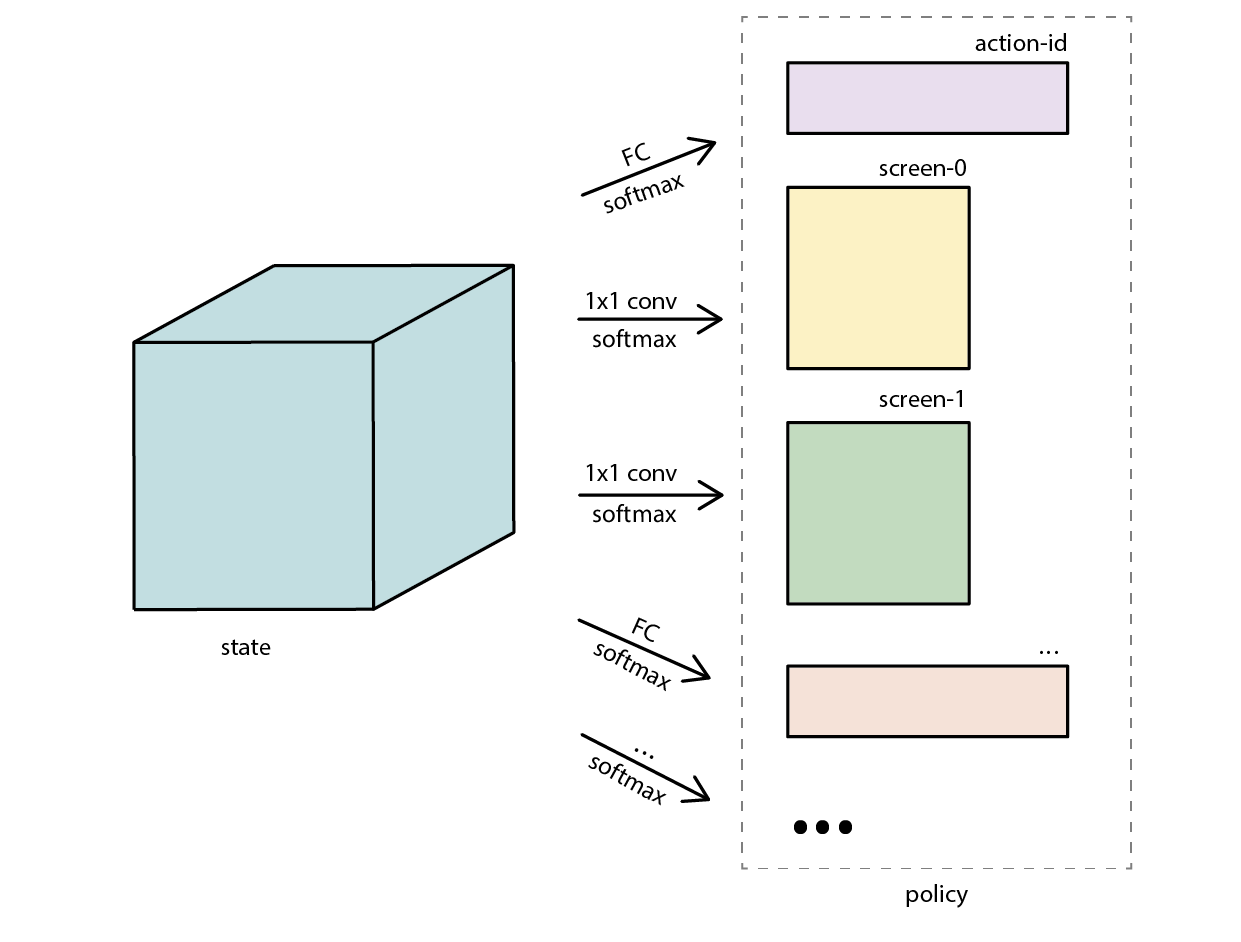
\includegraphics[width=\textwidth]{policy}
\caption{Action policy layer. State block is transformed into a spatial policy (used mainly for mouse-clicking on the screen) and non-spatial policy outputs. An output consist of probability distributions across possible values, such as action ids or specific pixels to click.}
\label{fig:policy}
\end{center}
\end{figure}

\section{Implementation Details}

Given that no official A2C paper was released, several sources of information were pooled for inspiration during development of this agent: the original A3C~\cite{mnih16} paper, it’s GPU support extension paper G-A3C~\cite{babaeizadeh2017ga3c}, the OpenAI baselines repository~\cite{baselines} and PyTorch based RL algorithms repository~\cite{pytorchrl}, both of which contained a reference A2C implementation. Earlier attempts to replicate SC2LE were also loosely referenced, however at the time of writing they were missing key aspects, relying on a different or incomplete architecture interpretation. Parts of the code that were most inspired by the attempts were marked with a reference link in the source code.
\\\\
Agent is implemented with the Python programming language and TensorFlow -- a general-purpose automatic differentiation library~\cite{Abadi2016}. With TensorFlow, complex differentiable layers can be defined seamlessly in a flexible computation graph. Derivatives of the layers are calculated automatically by applying the backpropagation algorithm. Additionally, NumPy~\cite{Oliphant2015} and SciPy~\cite{Jones2001} were used for helper methods during input/output preprocessing stages.
\\\\
Agent codebase is designed with ease of extension in mind, either with alternative algorithm implementations, model implementations or even with alternative Starcraft II communication methods (such as the upcoming raw pixel API). See Figure~\ref{fig:structure} below for a visualization of the codebase structure.
\\\\
Flexibility with regards to the choice of input features is key during experimentation step and lacking in alternative approaches. Here it is implemented as a list of accepted features stored in an external JSON configuration file which is loaded during initialization into a \texttt{Config} class instance, passed to \texttt{EnvPool} and \texttt{A2CAgent} instances.
\\\\
Model-free algorithms such as A2C require significant amount of samples to learn even the most basic policies, which is why codebase was structured with strong support for parallelization. API is defined such that the number of environments is hidden away from the agent or its model, which means that any number of environments can be supported, only limited by hardware capabilities. This is for the most part enabled with strong vectorization capabilities of TensorFlow and NumPy.
\\\\
Communication with the game engine is done through the \texttt{SC2Env} class from PySC2 library. Instances of \texttt{SC2Env} are created as separate processes and communicated with via the \texttt{EnvPool} class, based on the feature specification loaded into the \texttt{Config} class. \texttt{EnvPool} itself is wrapped with \texttt{EnvWrapper} which provides simple API for the agent to get relevant input features and provide necessary actions.
%\\\\
\\\\\
The main class of the codebase is the \texttt{A2CAgent}, which accepts the TensorFlow Session instance, \texttt{Config} instance and model definition as a lambda function defined in a separate class. This class is solely responsible both for acting and training of the agent. While having many responsibilities, content of the class was kept relatively short thanks to powerful vectorized operations support of TensorFlow.
\\\\
The glue between the agent and the environment is implemented in a lightweight \texttt{Runner} class, which essentially only contains the main execution loop and logging utilities.

\begin{figure}[ht]
\begin{center}
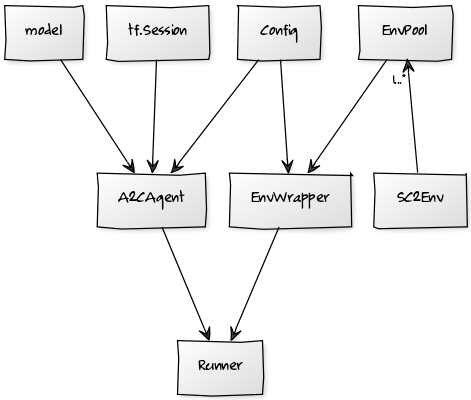
\includegraphics[width=0.7\textwidth]{structure}
\caption{Structure of the implemented codebase.}
\label{fig:structure}
\end{center}
\end{figure}